\chapter{عالم المتغيّرات}

تعلّمت كيفية إظهار نصّ على الشاشة. جيد، لكنّ هذا ليس شيئا مهماً. هذا لأنك لا تعرف بعد ما يدعى بـ\textbf{المتغيّرات}
(\textenglish{Variables})
في البرمجة.

فائدة هذه المتغيرات هي تمكين الحاسوب من حفظ أعداد في الذاكرة. سنبدأ ببعض الشرح حول ذاكرة الحاسوب وكيفيّة عملها. قد يبدو هذا بسيطا جدّا للبعض، لكنّي أفترض أنّك لا تعرف شيئا عن ذاكرة الحاسوب.

\section{أمر متعلق بالذاكرة}
ما سأعلمك في هذا الفصل هو أمر له علاقة مباشرة بذاكرة حاسوبك.

كل إنسان حيّ له ذاكرة. الأمر عينه بالنسبة للحاسوب، لكن الحاسوب له أنواع عديدة من الذاكرة.

\begin{question}
  لم يملك الحاسوب أنواع عديدة من الذاكرة، واحدة يمكنها أن تكفي، أليس الأمر كذلك ؟
\end{question}

كلّا : المشكلة أننا نحتاج ذاكرة سريعة (لاسترجاع المعلومات بسرعة) وفي نفس الوقت كبيرة (لحفظ بيانات كثيرة) قد تضحك إن أخبرتك أننا حتى اليوم لم نتمكن من صنع ذاكرة بهذه المواصفات. أو بالأحرى الذاكرة السريعة باهظة الثمن لذلك لا يتم إنتاج الكثير منها.

لذلك نجد في الحواسيب الحديثة ذاكرة سريعة جدا لكنها ليس ذات سعة كبيرة، وأخرى ذات سعة كبيرة جدّا لكنها غير سريعة.

\subsection{الأنواع المختلفة من الذاكرة}
كي أوضح لك الصورة أكثر، إليك أنواع الذاكرة الموجودة في الحاسوب، من الأسرع إلى الأبطأ :

\begin{enumerate}
  \item السجلات
  (\textenglish{Registers}) :
ذاكرة سريعة جدّا، موجودة داخل المعالج.
  \item ذاكرة التخبئة 
  (\textenglish{Cache memory}) :
تمثل همزة وصل بين السجلات والذاكرة الحية.
  \item ذاكرة الوصول العشوائي 
  (\textenglish{Random access memory}) :
و هي الذاكرة التي نستخدمها كثيرا، وتدعى اختصارا
\textenglish{RAM}.
  \item القرص الصلب
  (\textenglish{Hard disk}) :
والذي تعرفه بالطبع، نستعمله لحفظ الملفات.
\end{enumerate}

كما قلت لك، لقد رتبتها من الأسرع (السجلات) إلى الأبطأ (القرص الصلب)، وإن كنت قد تابعت جيدا فقد فهمت أن الذاكرة الأصغر هي الأسرع والأبطأ هي الأكبر.\\
السجلات لا تسع إلا لحمل بضعة أعداد أما القرص الصلب فيمكنه تخزين ملفات ضخمة.

\begin{information}
   عندما أقول ذاكرة بطيئة فهذا بالنسبة لحاسوبك، ففي نظر الحاسوب استغراق 8 ميلي ثانية للوصول إلى القرص الصلب يعتبر زمنا طويلا جدّا !
\end{information}

ما الذي يجب أن أتذكره من كل هذا ؟\\
أردت أن أخبرك أننا في الفصول القادمة سوف نستخدم ذاكرة الوصول العشوائي كثيرا. سنتعلم أيضا كيفية القراءة والكتابة في الملفات على القرص الصلب (ليس الآن، لا يزال الوقت مبكّرا على هذا). أمّا بخصوص السجلّات وذاكرة التخبئة فلن نتعامل معهما مطلقا، فالحاسوب هو من سيهتم بأمرهما.

\begin{information}
  في لغات البرمجة منخفضة المستوى، كلغة التجميع
(\textenglish{Assembly language})
نتعامل مباشرة مع السجلّات، لقد درستها، ويمكنني أن أقول لك أن القيام بعملية ضرب بسيطة يتطلب مجهودا ! لحسن الحظ ففي لغة
\textenglish{C}
 (وفي أغلب اللغات الأخرى) الأمر أسهل من ذلك بكثير.
\end{information}

يجب إضافة شيء مهمّ آخر : القرص الصلب هو الوحيد الذي يمكنه حفظ المعلومات بشكل دائم.
\textbf{كل أنواع الذاكرات الأخرى مؤقتة، فبمجرد إطفاء الحاسوب تفقد كل محتواها} !

لحسن الحظ، عند إعادة تشغيل الحاسوب، يقوم القرص الصلب بتذكيرها بمحتواها.

\subsection{صورة لذاكرة الوصول العشوائي}

نظرا لأننا سنستعمل ذاكرة الوصول العشوائي خلال لحظات، فمن الأفضل أن أريها لك (مؤطرة بالأحمر):

\begin{figure}[H]
	\centering
	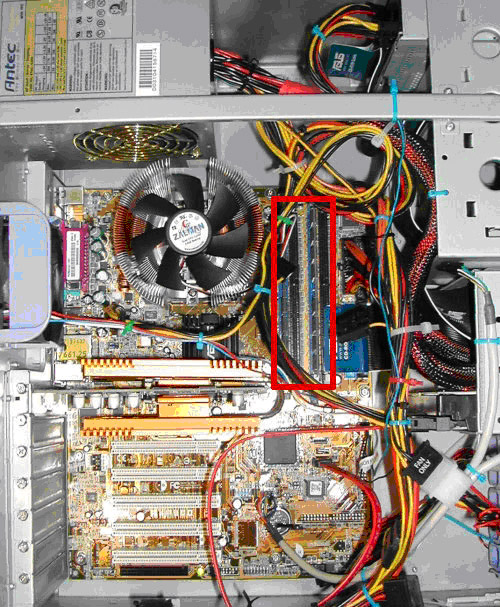
\includegraphics[width=0.8\textwidth]{Chapter_I-4_Computer}
\end{figure}

لا أطلب منك معرفة كيفية عملها، لكن أردت فقط أن أريك مكانها داخل جهازك. وهذه صورة مقربة لإحدى أشرطتها :

\begin{figure}[H]
	\centering
	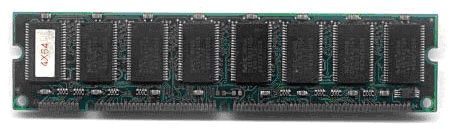
\includegraphics[width=0.8\textwidth]{Chapter_I-4_RAM}
\end{figure}

و هي تدعى اختصارا
\textbf{\textenglish{RAM}}،
لذلك لا تحتر إن سميتها هكذا لاحقا. بالنسبة للذاكرات الأخرى (السجلات والتخبئة) فهي صغيرة لدرجة أنه لا يمكن رؤيتها بالعين المجرّدة.

\subsection{مخطط ذاكرة الوصول العشوائي}

عرض المزيد من الصور لن يفيدك كثيرا، لكن يجب عليك فهم كيف تعمل من الداخل، لذلك سأقدم لك هذا المخطط البسيط الذي يمثل هندسة ذاكرة الوصول العشوائي :

\begin{figure}[H]
	\centering
	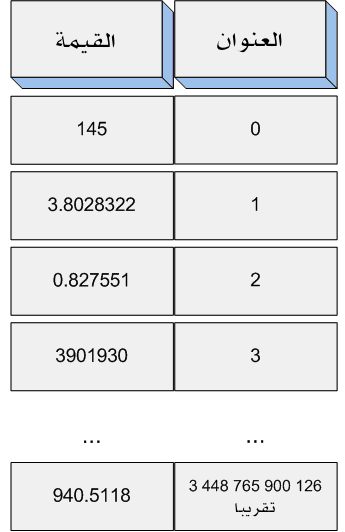
\includegraphics[width=0.5\textwidth]{Chapter_I-4_RAM-Schema}
\end{figure}


كما ترى، يمكننا أن نميز عمودين :

\begin{itemize}
  \item هناك
\textbf{العناوين}
: هي أعداد تسمح للحاسوب بتحديد موضع القيم في الـ\textenglish{RAM}
. نبدأ بالعنوان 0 وننتهي بالعنوان 3,448,765,900,126 وبعض الأجزاء. لا أعلم بالضبط كم عدد العناوين الموجودة في الـ\textenglish{RAM}
، لكني أعرف أنها كثيرة جدا. إضافة إلى ذلك، هذا أمر يتعلق بكمية الذاكرة الموجودة في جهازك، فكلما زادت الذاكرة زادت معها العناوين وصار بإمكاننا تخزين معلومات أكثر.
  \item عند كل عنوان يمكننا تخزين
\textbf{قيمة}
(عدد). حاسوبك يقوم بتخزين هذه الأعداد في ذاكرة الوصول العشوائي لكي يتمكن من تذكرها. ولا يمكننا تخزين سوى عدد واحد عند كل عنوان.
\end{itemize}

لا يمكن للذاكرة الحية تخزين شيء سوى الأعداد.

\begin{question}
  لكن كيف يمكننا تخزين الكلمات ؟
\end{question}

سؤال جيد. في الواقع حتى الحروف ليست سوى أعدادا في نظر الحاسوب ! الجملة هي مجرد تتابع لأعداد.\\
يوجد جدول يوافق بين الأعداد والحروف، جدول يقول مثلا بأن العدد 67 يوافق الحرف
\textenglish{Y}.
لن أدخل في التفاصيل أكثر، ستكون لنا فرصة للرجوع إلى هذا لاحقا.

فلنعد إلى مخططنا، الأمور بسيطة جدا : إذا أراد الحاسوب تذكر العدد 5 (الذي قد يمثل عدد الأرواح المتبقية لشخصية في لعبة) فسوف يضعه في مكان ما في الذاكرة أين يتوفر مكان شاغر ويحفظ العنوان الموافق (مثلا 3,062,199,902). لاحقا، عندما يريد معرفة هذا العدد فسيذهب إلى خانة الذاكرة التي تحمل العنوان رقم 3,062,199,902 وسيجد القيمة 5.

هذه آلية عمل الذاكرة بشكل عام. قد يكون الأمر لا زال غامضا في ذهنك حاليا (ما فائدة تخزين عدد إن كان علينا تذكر عنوانه بدلا من ذلك ؟) لكن كل شيء سيتضح مع بقية الفصول، أنا أعدك !

\section{التصريح عن متغير}

صدّقني هذه المقدّمة القصيرة عن الذاكرة ستكون مهمّة أكثر مما تعتقد. الآن يمكننا العودة إلى البرمجة.

إذن، ما هو
\textbf{المتغير}
(\textenglish{Variable}) ؟\\
إنه معلومة صغيرة نخزنها مؤقتا في الذاكرة الحية. ببساطة يمكننا القول إن المتغير هو قيمة يمكن أن تتغير أثناء اشتغال البرنامج. مثلا عددنا 5 الذي ذكرناه سابقا يمكن أن يتناقص بمرور الزمن. إذا وصل إلى العدد 0 فسنعرف أن اللاعب قد خسر.

في برامجنا سيكون هناك الكثير من المتغيرات. ستراها في كلّ مكان.

في لغة الـ\textenglish{C}،
 المتغير يتميز بشيئين :

\begin{itemize}
  \item \textbf{قيمة}
: هو العدد الذي يحويه، $ 5 $ مثلا.
  \item \textbf{اسم}
: وهو الذي يمكننا من معرفة المتغيّر. في البرمجة لن يكون علينا تذكّر عناوين الذاكرة. بدلا من ذلك علينا فقط استخدام أسماء المتغيرات. المترجم هو من سيقوم بتحويل الأسماء إلى عناوين.
\end{itemize}

\subsection{إعطاء اسم للمتغير}

في لغة البرمجة
\textenglish{C}
كل متغير يجب أن يملك اسما خاصا به. ومن أجل متغيرنا الذي يحوي عدد الأرواح المتبقية للاعب يمكننا أن نسميه
"\textenglish{Number of lives}"
أو شيء من هذا القبيل.

للأسف توجد بعض الشروط، لا يمكنك تسمية المتغير كيفما شئت :

\begin{itemize}
  \item لا يجب أن يحتوي الاسم سوى على الحروف الصغيرة والكبيرة والأرقام
(\InlineCode{abcABC012}).
  \item يجب أن يبدأ الاسم بحرف.
  \item المسافات ممنوعة. بدلا من ذلك يمكننا استخدام الحرف المعروف باسم
\textenglish{underscore}
 (\InlineCode{\_}).
إنه الحرف الخاص الوحيد غير الحروف والأرقام الذي يمكن استعماله في اسم متغير.
  \item لا يمكنك استخدام حروف غير الحروف الإنجليزية.
\end{itemize}

وأخيرا يجب أن تعرف أن لغة
\textenglish{C}
 تفرّق بين الحروف الصغيرة والكبيرة. ولثقافتك، نقول إن
\textenglish{C}
 حساسة لحالة الحروف
(\textenglish{Case sensitive}).
كمثال، الأسماء
\InlineCode{width}
 أو
\InlineCode{WIDTH}
 أو
\InlineCode{WiDth}
تعتبر أسماء متغيرات مختلفة، حتى لو كانت تعني لنا الأمر نفسه.

هذه أمثلة عن أسماء متغيرات صالحة :
\InlineCode{numberOfLives}،
\InlineCode{name}،
\InlineCode{surname}،
\InlineCode{phone\_number}،
\InlineCode{phoneNumber}.

لكل مبرمج طريقة خاصة في كتابة أسماء المتغيرات. خلال هذا الفصل سأريك طريقتي :

\begin{itemize}
  \item أبدأ دائما بحرف صغير.
  \item إن كان في الاسم أكثر من كلمة أضع حرف كبيرا في بداية كلّ كلمة.
\end{itemize}

أطلب منك كتابة أسماء متغيراتك بنفس الطريقة التي أتبعها، هذا لكي نكون على تفاهم.

\begin{critical}
  أيّا كان اختيارك، فعليك دائما إعطاء أسماء واضحة لمتغيراتك. كان بإمكاننا اختصار
\InlineCode{numberOfLives}
إلى
\InlineCode{nol}
مثلا. هذا أقصر في الكتابة، لكنه أقل وضوحا عندما تعيد قراءة الشفرة المصدرية. فأنصحك بإعطاء أسماء أطول لمتغيراتك إن كان ذلك يحسّن فهمها.
\end{critical}

\subsection{أنواع المتغيرات}

حاسوبنا كما نعلم ليس سوى آلة كبيرة جدا للحساب. لا يجيد التعامل سوى مع الأعداد. لكن يوجد أنواع كثيرة من الأعداد :

\begin{itemize}
  \item الأعداد الصحيحة الموجبة (الطبيعية) مثل :$ 45 $، $ 398 $، $ 7650 $.
  \item الأعداد العشرية، أي التي تحوي فاصلة عشرية : $ 75.909 $، $ 1.7741 $، $ 9810.7 $.
  \item الأعداد الصحيحة السالبة : $ -87 $، $ -916 $.
  \item الأعداد العشرية السالبة : $ -76.9 $، $ -100.11 $.
\end{itemize}

حاسوبك المسكين بحاجة للمساعدة ! عندما تطلب منه تخزين عدد، يجب أن تذكر له نوعه. هذا ليس لأنّه لا يمكنه التعرف عليه تلقائيّا، ولكن للتنظيم ولعدم أخذ كميات كبيرة من الذاكرة بدون فائدة.

عندما تصرّح عن متغيّر فسيكون عليك تحديد نوعه. إليك أنواع المتغيرات الأساسية في لغة \textenglish{C} :

\begin{Table}{3} % The number of columns is required (here is 3)
  النوع & الحد الأدنى & الحد الأقصى\\
  \LR{\ttfamily signed char} & $-128$ & $127$ \\
  \LR{\ttfamily int} & $-32,768$ & $32,767$ \\
  \LR{\ttfamily long} & $-2147483648$ & $2147483647$ \\
  \LR{\ttfamily float} & $-1 \times 10^{37}$ & $1 \times 10^{37}-1$\\
  \LR{\ttfamily double} & $-1 \times 10^{37}$ & $1 \times 10^{37}-1$\\
\end{Table}

\begin{warning}
  القيم المعروضة هنا تمثل الحد الأدنى المضمون من طرف اللغة. في الحقيقة قد تتمكن من تخزين أعداد أكبر من هذه. في كلّ الأحوال من المستحسن تذكّر هذه القيم عندما تختار نوع متغيراتك.
\end{warning}

\begin{information}
  للعلم أنّي لم أعرض جميع الأنواع هنا، بل الأساسية منها فقط.
\end{information}

الأنواع الثلاثة الأولى
(\InlineCode{char}، \InlineCode{int}، \InlineCode{long})
تسمح يتخزين الأعداد الصحيحة ($ 1 $، $ 2 $، $ 3 $، $ 4 $، \dots).\\
النوعان الأخيران
(\InlineCode{float}، \InlineCode{double})
يسمحان بتخزين الأعداد العشرية ($ 13.8 $، $ 16.911 $ \dots).

سترى أنّنا نتعامل من الأعداد الصحيحة معظم الوقت لأنّها سهلة الإستخدام.

\begin{critical}
  احذر في الأعداد العشرية من استخدام الفاصلة، حاسوبك لا يستخدم سوى النقطة. لذلك لا تكتب
$54,9$
 بدل
$54.9$ !
\end{critical}

هذا ليس كلّ شيء، توجد أنواع أخرى تعرف بـ\InlineCode{unsigned}
 (عديمة الإشارة) تصلح لتخزين الأعداد الموجبة فقط. يجب إضافة كلمة
\InlineCode{unsigned}
إلى النوع لاستخدامها.

\begin{Table*}{2}
  \LR{\ttfamily unsigned char} & من
$0$
 إلى
$255$ \\
  \LR{\ttfamily unsigned int} & من
$0$
إلى
$65,535$ \\
  \LR{\ttfamily unsigned int} & من
$0$
إلى
$4,294,967,295$\\
\end{Table*}

كما ترى، مشكلة الأنواع عديمة الإشارة هي عدم القدرة على تخزين الأعداد السالبة، لكن الشيء الإيجابي هي أنّها توفّر لنا ضعف حجم التخزين لكلّ نوع موافق (مثلا
\InlineCode{signed char}
يتوقّف عند 127، بينما
\InlineCode{unsigned char}
يمتد إلى 255).

\begin{information}
  تلاحظ أنّ النوع
\InlineCode{char}
قد تمّ إدراجه إمّا مع الكلمة المفتاحية
\InlineCode{signed}،
أو مع الكلمة المفتاحية
\InlineCode{unsigned}
لكن لا يوضع وحده أبدا. السبب بسيط : هذا النوع يمكن أن يكون بإشارة أو بدون إشارة حسب الحواسيب. لذلك أنصحكم بتحديد أي واحد منهما تريدون حسب نوع القيمة المراد تخزينها.
\end{information}

\begin{question}
  لِمَاذا توجد ثلاثة أنواع من المتغيرات الصحيحة ؟ ألا يكفي نوع واحد ؟
\end{question}

بلى، و لكن إنشاء أنواع متعدّدة هدفه الاقتصاد من استهلاك الذاكرة. فعندما نطلب من الحاسوب حجز مساحة لمتغيّر من نوع
\InlineCode{char}
فهذا سيكون أقل من المساحة المستهلكة لو إخترنا متغيّرا من نوع
\InlineCode{int}.

كان هذا مهمّا جدّا عندما كانت الحواسيب محدودة الذاكرة. أمّا اليوم فحواسيبنا بها ذاكرات كبيرة جدّا فلم يعد هذا يمثّل مشكلة. إذا احترت أيّ واحد من الأنواع تستخدم، فاختر
\InlineCode{int}
للأعداد الصحيحة (أو
\InlineCode{double}
للعشرية).

باختصار، نقوم بالتفريق خاصّة بين الأعداد الصحيحة و العشريّة
\begin{itemize}
  \item بالنسبة للأعداد الصحيحة، نستعمل عادة
\InlineCode{int}.
  \item بالنسبة للأعداد العشريّة نستعمل عادة
\InlineCode{double}.
\end{itemize}

\subsection{التصريح عن متغيّر}
ها قد بدأنا. الآن سنقوم بإنشاء برنامج كونسول نسميه "\textenglish{variables}".\\
 سنتعلم كيف نصرّح عن متغيّر، أي
 \textbf{الطلب من الحاسوب إذنا باستخدام شيء من ذاكرة الوصول العشوائي}.

 التصريح سيكون سهلا الآن، يجب علينا فقط أن نتّبع الترتيب التالي :
 
 \begin{enumerate}
   \item نحدّد نوع المتغيّر المراد إنشائه.
   \item نترك فراغا.
   \item نحدد اسم المتغيّر.
   \item و أخيرا، يجب ألاّ ننسى أبدا وضع الفاصلة المنقوطة.
 \end{enumerate}

 مثلا، إذا أردنا إنشاء المتغيّر
\InlineCode{numberOfLives}
 من نوع
\InlineCode{int}
سنكتب السطر التالي :

\begin{Csource}
int numberOfLives;
\end{Csource}

هذا كل ما في الأمر، وإليك بعض الأمثلة الغبيّة لملاحظة الشكل :

\begin{Csource}
int mathMark;
double moneySumReceived;
unsigned int numberOfReadersWhoAreReadingALongVariableName;
\end{Csource}

حسنا، أعتقد أنّك فهمت المبدأ الآن !

ما فعلناه للتو يسمّى
\textbf{تصريحا عن متغيّر}
(\textenglish{Declaring a variable})
(هذا مصطلح يجب حفظه). يمكنك وضع التصريحات في بدايات الدوال. و بما أن لدينا دالّة وحيدة فقط
(الدالة
\InlineCode{main})
فسنصرّح المتغيّر هكذا :

\begin{Csource}
#include <stdio.h>
#include <stdlib.h>

int main(int argc, char *argv[]) // Equivalent to int main()
{
  int numberOfLives;

  return 0;
}
\end{Csource}

إن قمتم بتشغيل البرنامج فستلاحظ بدهشة 
\dots
أنّه لا يقوم بشيء.

\subsection{بعض التوضيحات}

في الواقع، هناك أشياء تحدث، لكنّك لا تراها. عندما يصل البرنامج إلى سطر التصريح عن المتغيّر فإنّه يطلب من الحاسوب بهدوء أن يعطيه شيئا من ذاكرة الوصول العشوائي.\\
إن تم كلّ شيء على أحسن حال (و هذا ما يقع في غالب الأحيان) فإن الحاسوب يوافق على هذا الطلب.
المشكل الوحيد الذي يمكن أن يقع هو امتلاء الذاكرة، لكنّ هذا أمر نادر الحدوث، من الذي سيملؤ الذاكرة بمتغيرات
\InlineCode{int}
 ؟

لذلك كن متيقناً أنه سوف يتم إنشاء المتغيرات بنجاح.

\begin{information}
  معلومة صغيرة : إن كان لديك عدد من المتغيّرات بنفس النوع تريد التصريح عنها، فمن غير الضروري كتابة سطر لكلّ متغيّر. يكفي فصل أسماء المتغيّرات عن بعضها بفواصل على نفس السطر، مثلا~:
\InlineCode{int numberOfLives, level, playerAge;}.
هذا ينشئ ثلاثة متغيّرات أسماؤها على التوالي :
\InlineCode{numberOfLives}، \InlineCode{level}
و
\InlineCode{playerAge}.
\end{information}

و الآن يجب علينا إعطاء قيمة للمتغيّر الذي أنشأناه.

\subsection{إسناد قيمة إلى متغيّر}
هذا أمر سهل للغاية فإن أردنا أن نعطي قيمة لمتغيرنا
\InlineCode{numberOfLives}
فيكمننا ببساطة كتابة هذا :

\begin{Csource}
numberOfLives = 5;
\end{Csource}

لن نفعل شيئا بعد هذا. ستضع اسم المتغير، إشارة تساوي، بعدها القيمة التي تريد أن تضعها بالداخل، في هذه الحالة سنعطي القيمة 5 للمتغير
\InlineCode{numberOfLives}.
برنامجنا الكامل سيكون هكذا :

\begin{Csource}
#include <stdio.h>
#include <stdlib.h>

int main(int argc, char *argv[]) // Equivalent to int main()
{
  int numberOfLives;
  numberOfLives = 5;

  return 0;
}
\end{Csource}

هنا أيضا لا شيء يُعرض على الشاشة، كلّ شيء يحدث في الذاكرة.\\
في أعماق الحاسوب هناك خانة ذاكرة تأخذ القيمة 5. أليس شيئا رائعا ؟

يمكننا أن نستمتع بتغيير القيمة :

\begin{Csource}
int numberOfLives;
numberOfLives = 5;
numberOfLives = 4;
numberOfLives = 3;
\end{Csource}

في هذا المثال، المتغير سيأخذ القيمة 5 ثم 4 ثم 3. و بما أنّ الحاسوب سريع جدّا ففي أقلّ من رمشة عين يأخذ المتغيّر القيم 5 ثمّ 4 ثمّ 3 ثمّ ينتهي البرنامج.

\subsection{قيمة متغيّر جديد}

هناك سؤال مهمّ يجب أن أطرحه عليك :

\begin{question}
  عند التصريح عن متغيّر، أيّ قيمة تكون فيه ؟
\end{question}

عندما يقرأ الحاسوب هذا السطر :

\begin{Csource}
int numberOfLives;
\end{Csource}

فسيحجز مكانا في الذاكرة لهذا المتغيّر، لكن ما هي قيمته في هذه اللحظة ؟\\
هل يملك قيمة افتراضيّة ؟ (0 مثلا).

الجواب هو لا، لا و لا ثمّ لا ! لا توجد قيمة افتراضيّة. المكان محجوز لكنّ القيمة لا تتغيّر. لا يتمّ حذف ما يوجد في خانة الذاكرة. ستكون قيمة متغيّرك هي نفس القيمة التي كانت موجودة من قبل في تلك الخانة، و
\textbf{يمكن أن تكون أيّ شيء} !

إن لم يتم تغيير هذا المكان من الذاكرة من قبل، فقد تكون قيمته 0، لكنّ هذا ليس مؤكّدا، قد يأخد متغيّرك القيمة 363 أو 18، و هذا يدلّ على بقايا برنامج قد استخدم هذه الخانة من قبل.\\
و لهذا كي لا تعترضنا المشاكل لاحقا يجب تهيئة المتغير عند التصريح عنه، في لغة
\textenglish{C}
هذا أمر ممكن حيث أنّ كل ما يجب القيام به هو الدمج بين التصريح و تعيين قيمة المتغير في نفس التعليمة كالتالي :

\begin{Csource}
int numberOfLives = 5;
\end{Csource}

هنا يتمّ  التصريح عن المتغيّر ثمّ إسناد قيمة 5 له بطريقة مباشرة.\\
الشيء الإيجابي هنا أننا متأكدون من أنّ المتغيّر يحمل القيمة 5 مبدئيّا.

\subsection{الثوابت}

قد نريد أحيانا إنشاء متغيّر يحمل قيمة ثابتة طوال وقت تشغيل البرنامج. هذا يعني أنّه بمجرّد التصريح عنه، فإنّه يحافظ على قيمته و لا يمكن لأحد تغيير قيمته التي يحويها.

هذا النوع الخاص من المتغيّرات يسمى الثوابت (\textenglish{Constants})، طبعا هذا لأنّ قيمتها تبقى ثابتة.

للتصريح عن ثابت، تكفي إضافة كلمة
\InlineCode{const}
قبل نوع المتغيّر. و لكن يجب إعطاء الثابت قيمة بمجرّد التصريح عنه، لأنّه لاحقا سيكون الوقت متأخّرا و لن نتمكّن من تغيير قيمته.

مثال على التصريح بثابت :

\begin{Csource}
const int INITIAL_NUMBER_OF_LIVES = 5;
\end{Csource}

\begin{information}
  ليس من الضروري أن يكون اسم الثابت مكوّنا من حروف كبيرة فقط، لكنّ هذا يساعدنا على التفريق بينها و بين المتغيّرات. لاحظ أيضا أننا نستخدم الرمز
\_
 بدلا من الفراغ.
\end{information}

بغضّ النظر عن هذا، الثابت يستعمل بشكل عادي كالمتغير ، يمكنك عرض قيمته إن أردت. الفرق الوحيد هو أنّه إذا حاولت تغيير قيمة الثابت في برنامجك فسينبّهك المترجم إلى وجود خطأ.

أخطاء الترجمة تعرض أسفل الشاشة (في المكان الذي أسميه "منطقة الموت" هل تتذكر ؟)، في هذه الحالة سيقوم المترجم بعرض رسالة تشبه التالي :\\
\InlineCode{[Warning] assignment of read-only variable 'INITIAL\_NUMBER\_OF\_LIVES'}

\section{عرض محتوى متغير}

نحن نعرف كيف نعرض نصّا على الشاشة باستخدام الدالة
\InlineCode{printf}.\\
الآن سنتعلم كيف نعرض القيمة الخاصة بالمتغير باسخدام نفس الدالة.

سنستخدم الدالة
\InlineCode{printf}
بنفس الطريقة، باستثناء أننا سنقوم بإضافة رمز خاص في المكان الّذي نريد عرض قيمة المتغيّر فيه. مثلا :

\begin{Csource}
printf("You have %d lives left");
\end{Csource}

هذا الرمز الخاص ما هو إلّا
\InlineCode{\%}
 متبوعا بمحرف
(\InlineCode{'d'}
في هذا المثال). هذا الحرف يبيّن ما الذي سنقوم بعرضه.
\InlineCode{'d'}
تعني أننا سنعرض قيمة متغيّر من نوع
\InlineCode{int}.\\
توجد حروف أخرى عديدة، لكن من أجل التبسيط فسنكتفي بهذه :

\begin{Table}{2}
الشكل & النوع المنتظر\\
\LR{\ttfamily \%d} & \LR{\ttfamily int}\\
\LR{\ttfamily \%ld} & \LR{\ttfamily long}\\
\LR{\ttfamily \%f} & \LR{\ttfamily float}\\
\LR{\ttfamily \%f} & \LR{\ttfamily double}\\
\end{Table}

\begin{information}
  لاحظ أنّ الشكل المستخدم لعرض
\InlineCode{float}
و
\InlineCode{double}
هو نفسه.
\end{information}
سأعلّمك رموزا أخرى في الوقت المناسب، حاليّا تذكّر هذه فقط.

شارفنا على الإنتهاء. حددنا موضع كتابة عدد صحيح، لكننا لم نذكر ما هو ! يجب علينا أن نحدد للدالة
\InlineCode{printf}
المتغيّر الذي نريد عرض قيمته.\\
لفعل ذلك، أكتب اسم المتغيّر بعد علامات الاقتباس بعد وضع فاصلة :
\begin{Csource}
printf("You have %d lives left", numberOfLives);
\end{Csource}
\InlineCode{\%d}
 سيتمّ استبداله بقيمة المتغيّر المكتوب بعد الفاصلة، أي
\InlineCode{numberOfLives}.\\
فلنجرّب هذا في برنامج :

\begin{Csource}
#include <stdio.h>
#include <stdlib.h>

int main(int argc, char *argv[])
{
  int numberOfLives = 5; // The player has 5 lives in the beginning.

  printf("You have %d lives left\n", numberOfLives);
  printf("**** B A M ****\n"); // A big blow on his head.
  numberOfLives = 4; // Life lost
  printf("Sorry, only %d lives are remaining now !\n\n", numberOfLives);

  return 0;
}
\end{Csource}

يمكن أن يكون البرنامج قاعدة للعبة فيديو (ينقصه الخيال فقط).\\
هذا البرنامج يعرض على الشاشة :

\begin{Console}
You have 5 lives left
**** B A M ****
Sorry, only 4 lives are remaining now !

\end{Console}

يجب أن تفهم ما الذي يحدث في البرنامج :

\begin{enumerate}
  \item في البداية يملك اللاعب 5 أرواح، نعرض هذا في
\InlineCode{printf}.
  \item  بعدها يتلقى اللاعب ضربة على رأسه (في مكان
\textenglish{BAM}).
  \item بعدها لا يبقى له سوى 4 أرواح، نعرض هذا أيضا باستخدام
\InlineCode{printf}.
\end{enumerate}

كان ذلك سهلا !

\subsection{عرض عدّة متغيّرات باستخدام \texttt{printf} واحدة}

يمكن عرض قيم متغيرات عديدة بنفس الدالة
\InlineCode{printf}.
يكفي فقط أن تضع
\InlineCode{\%d}
أو
\InlineCode{\%f}
 في الأمكنة المناسبة، ثم تحديد المتغيّرات الموافقة بنفس الترتيب، مفصولة عن بعضها البعض بفواصل.

مثال :

\begin{Csource}
printf("You have %d lives and you are in the level n° %d", numberOfLives, level);
\end{Csource}

\begin{warning}
  يجب عليك تحديد المتغيّرات بالترتيب الصحيح،
\InlineCode{\%d}
الأولى توافق المتغيّر الأوّل
(\InlineCode{numberOfLives})
و
\InlineCode{\%d}
الثانية توافق المتغيّر الثاني
(\InlineCode{level}).
إذا أخطأت في الترتيب، فلن يكون للجملة أيّ معنى.
\end{warning}

حسنا، فلنقم بتجربة صغيرة الآن. لاحظ أنني قد حذفت توجيهات المعالج القبلي (أعني تلك السطور التي تبدأ برمز
\InlineCode{\#})،
أنا أفترض أنك تضعها في كلّ مرّة الآن :

\begin{Csource}
int main(int argc, char *argv[])
{
  int numberOfLives = 5, level = 1;

  printf("You have %d lives and you are in the level n° %d", numberOfLives, level);

  return 0;
}
\end{Csource}

و هذا يعرض لك :

\begin{Console}
You have 5 lives and you are in the level n° 1
\end{Console}

\section{استرجاع إدخال}

بدأت المتغيرات تصبح ممتعة الآن. سنتعلم كيف نطلب من المستخدم كتابة عدد في الكونسول. سنسترجع هذا العدد و نحفظه في متغير. عندما نفعل ذلك سيكون بإمكاننا القيام بكثير من الأمور، سوف ترى ذلك.

لكي نطلب من المستخدم إدخال شيء سنقوم باستخدام دالة جاهزة تسمّى :
\InlineCode{scanf}.\\
هذه الدالة تشبه إلى حد كبير
\InlineCode{printf}.
يجب عليك وضع شكل لتحديد ما سيدخله المستخدم
(\InlineCode{int}، \InlineCode{float} \dots).
ثم يجب عليك تعيين إسم المتغير الذي سيأخذ هذا العدد.

هذا ما سنفعله على سبيل المثال :

\begin{Csource}
int age = 0;
scanf("%d", &age);
\end{Csource}

علينا وضع
\InlineCode{\%d}
بين مزدوجتين. كما يجب وضع
\InlineCode{\&}
أمام اسم المتغيّر الذي سيستقبل القيمة.

\begin{question}
  و لكن لماذا نضع
\InlineCode{\&}
أمام اسم المتغيّر ؟
\end{question}

هنا يجب عليك أن تثق بي. لأنه لا يمكنني أن أشرح لك ما الذي تعنيه في الوقت الحالي. لكني أضمن لك أنيّ سأقوم بشرحه في وقت لاحق.

\begin{critical}
احذر ! يوجد اختلاف صغير في الشكل بين
\InlineCode{printf}
و
\InlineCode{scanf}
 ! لاسترجاع
\InlineCode{float}
يجب استخدام الشكل
\InlineCode{"\%f"}،
أما من أجل النوع
\InlineCode{double}
 فيتم استخدام
\InlineCode{"\%lf"}.
\end{critical}

\begin{Csource}
double weight = 0;
scanf("%lf", &weight);
\end{Csource}

فلنعد إلى برنامجنا. عندما يصل هذا الأخير إلى
\InlineCode{scanf}،
يتوقف مؤقّتا منتظرا المستخدم لكي يدخل عددا. هذا العدد يتم حفظه في المتغير
\InlineCode{age}.
إليك برنامجا يطلب عمر المستخدم ثم يقوم بعرضه :

\begin{Csource}
int main(int argc, char * argv[])
{
  int age = 0;

  printf("How old are you ? ");
  scanf("%d", &age);
  printf("Ah ! so you are %d years old !\n\n", age);

  return 0;
}
\end{Csource}

و هذا ما يعرضه :

\begin{Console}
How old are you ? 20
Ah ! so you are 20 years old !

\end{Console}

يتوقف البرنامج مؤقّتا بعد عرض السؤال و يظهر مؤشرا على الشاشة، عليك إذن أن تكتب عددا (عمرك). اِضغط بعدها على المفتاح "إدخال"
(\textenglish{Enter}).
بعد ذلك يواصل البرنامج عمله. هنا، يقوم البرنامج بعرض قيمة المتغيّر
\InlineCode{age}
على الشاشة.

حسنا، لقد فهمت الأساس. بفضل الدالة
\InlineCode{scanf}
 يمكننا البدء في التفاعل مع المستخدم.

 ليكن في علمك أنه لا مانع من إدخال أي شيء غير عدد صحيح :
 
 \begin{itemize}
   \item إن قمت بإدخال عدد عشري، مثلا 2.9، فسيتم قطعه تلقائيّا. في هذه الحالة سيتم حفظ العدد 2 في المتغيّر.
   \item إن قمت بكتابة أحرف عشوائية، مثلا :
\textenglish{éèdyf}،
فلن تتغيّر قيمة المتغيّر. و الشيء الجيّد في هذه الحالة هو أننا قمنا بتهيئة قيمة المتغير على 0. لذلك سيعرض البرنامج :
"\textenglish{Ah ! so you are 0 years old}"
 إن لم يتم الأمر بشكل صحيح. لو لم نقم بتهيئة المتغيّر فسيعرض البرنامج عددا عشوائيا !
 \end{itemize}

\section*{ملخّص}

\begin{itemize}
  \item حواسيبنا تملك عدة أنواع من الذاكرة. من الأسرع إلى الأبطأ : السجلّات، ذاكرة التخبئة، الذاكرة الحيّة و القرص الصلب.
  \item للاحتفاظ بالمعلومات، يحتاج برنامجنا إلى تخزين البيانات في الذاكرة. لهذا يستخدم
\textbf{الذاكرة الحية}.
السجلّات و ذاكرة التخبئة تستخدم أيضا لزيادة الأداء، لكنّ هذا يحدث تلقائيا و ليس علينا أن نهتم بهذا الأمر.
  \item في الشفرة المصدرية،
\textbf{المتغيّرات}
هي البيانات المحفوظة مؤقّتا في الذاكرة الحيّة. قيمة هذه البيانات يمكن أن تتغيّر أثناء تشغيل البرنامج.
  \item بالمقابل، نطلق اسم
\textbf{الثوابت}
على بيانات محفوظة في الذاكرة الحيّة. قيمة هذه البيانات لا يمكن أن تتغيّر.
  \item توجد أنواع عديدة من المتغيّرات، تختلف في حجم الذاكرة التي تشغله. بعض الأنواع مثل
\InlineCode{int}
تستخدم لتخزين عدد صحيح، و أخرى مثل
\InlineCode{double}
تخزّن أعدادا عشريّة.
  \item الدالة
\InlineCode{scanf}
 تمكّننا من طلب عدد من المستخدم.
\end{itemize}
